\chapter{2DJ Estimation for Pure Shift NMR}
\label{chap:cupid}
Two key features of the \ac{NMR} experiment for which improvements are
constantly being sought are sensitivity and resolving power.
\correction{
    \label{corr:ns}
    There are numerous means of enhancing sensitivity, such as the use of
    magnets with higher field strengths ($\operatorname{SNR} \propto
    B_0^{3/2}$)~\cite{Maeda2019} and cryogenic probes~\cite{Kovacs2020}, as
    well as simply increasing the number of transients ($\operatorname{SNR}
    \propto N_{\text{t}}^{1/2}$)~\cite[Section 5.2]{Levitt2007}.
}
However, few means of achieving better resolution exist beyond increased field
strengths (resolution $\propto B_0$), and ensuring that a magnetic
field with a high degree of homogeneity is used through the use of shimming.
Significant interest has therefore
been given to the development of techniques which generate broadband homodecoupled
(\emph{pure shift}) spectra, in which the effects of homonuclear scalar
couplings are absent from the data. While often valuable for structural
assignment purposes, the influence of scalar couplings can lead to spectra
which are too crowded for meaningful insights to be gleaned. While it is
commonplace to decouple heteronuclear couplings at the point of \ac{FID}
acquisition~\cite{Shaka1983a, Shaka1983b,Shaka1985}, homonuclear decoupling is
far more challenging. At the time of writing, there are a number of approaches
for acquiring pure shift spectra; the most popular modern approach
involves running a suitable \ac{2D} pulse sequence, and concatenating the initial
sections of each \ac{FID}, in a process referred to as
\emph{chunking}~\cite{Meyer2013,Adams2014,Zangger2015}. The key drawback of all of
these techniques is that the resultant pure shift signal is considerably less
sensitive relative to a standard pulse-acquire experiment, since only a
fraction of the available spin magnetisation contributes to that which is
incorporated into the dataset.

In this chapter, a method for deriving pure shift spectra indirectly via the
estimation of \ac{2DJ} datasets is presented, which has been named
\acfi{CUPID}. It is illustrated that by extracting the parameters which
describe a \ac{2DJ} dataset, a pure shift spectrum with desirable
absorption-mode lineshapes can be produced without the signal loss associated
with experimental pure shift methods.

\section{Pure Shift NMR}

\subsection{The \acl{2DJ} Experiment}
The \ac{2DJ} experiment\cite{Aue1976, Morris2009} provided the first means of
achieving pure shift spectra. It has a simple pulse sequence, presented in
Figure \ref{fig:pure_shift_seqs}.a; after excitation of magnetisation onto the
transverse plane, the indirect dimension evolution consists of a spin echo, with
acquisition following immediately afterwards. Fourier transformation in both
dimensions leads to a spectrum in which only scalar couplings contribute in
$\Fone$, as the chemical shifts are refocussed by the spin echo, while both
scalar couplings and chemical shifts contribute in $\Ftwo$.
Peaks belonging to a particular multiplet lie along a line at \ang{45} to the
$F^{(1)}$ and $F^{(2)}$ axes, as seen in panel a. of Figure
\ref{fig:jres_spectrum}.
\begin{figure}%
    \centering%
    \includegraphics{jres_spectrum/jres_spectrum.pdf}%
    \caption[
        Example of a simple \acs{2DJ} spectra derived from an AMX spin system,
        processes in different ways.
    ]
    {%
        Example of a simple \acs{2DJ} spectrum derived from an AMX spin system.
        Each panel showcases the appearance of the spectrum following different
        processing procedures. Below: contour plots of the spectrum. Above: the
        summation of the spectrum along the indirect axis.
        \note{Put 45 line on panel a}
        \textbf{a.} Spectrum produced from sine-bell apodisation followed by
        \ac{FT} in both dimensions, which features phase-twist peaks, and which
        sums to zero along the indirect dimension. Each multiplet lies along a
        line at \ang{45} to the $F^{(1)}$ and $F^{(2)}$ axes. Note that this
        line often appears to make an angle that is greater than \ang{45} with
        the $F^{(2)}$ axis when viewing spectra, due to the relative scaling of
        the frequency axes (typically, $\fswtwo \gg \fswone)$.
        \textbf{b.} Magnitude-mode spectrum produced from \textbf{a.} by
        subjecting each point to $\sqrt{\Re(x)^2 + \Im(x)^2}$.
        \textbf{c.} Spectrum generated after application of a \ang{45} shear to
        \textbf{b}.  The summation produces a pure shift spectrum, though this
        features peaks with broad wings, and significant non-linearities.
   }%
    \label{fig:jres_spectrum}%
\end{figure}%

An FID generated by the \ac{2DJ} experiment is hypercomplex, taking the form of
\eqref{eq:general-fid} with $D=2$ and $\zeta^{(1)} = \exp(\iu\cdot)$, i.e.
\begin{equation}%
    \begin{split}%
        \jresfid\idxnonentwo =
        \sum_{m=0}^{M-1} \bdam \exp\left( \iu \bdphim \right)
            \exp\left(\left(2 \pi \iu \bdfonem
            - \bdetaonem\right) {\none}_{\vphantom{t}} \Dtone\right) \times \\
            \exp\left(\left(2 \pi \iu  \left(
            \bdftwom - \fofftwo \right)
            - \bdetatwom\right) {\ntwo}_{\vphantom{t}} \Dttwo\right)
            + \symbf{W}\left[n^{(1)}, n^{(2)}\right].
    \end{split}%
    \label{eq:jres-fid}
\end{equation}%
The transmitter offset term has been neglected in the indirect dimension, since
chemical shift evolution does not occur.
For each signal in the \ac{FID}, the indirect- and direct-dimension
frequencies are intimately linked by the relations
\begin{subequations}
    \begin{gather}
        \bdfonem = d_m,\\
        \bdftwom = c_m + d_m,
    \end{gather}
    \label{eq:f1-f2-2dj}
\end{subequations}
where $c_m$ is the Larmor frequency of the spin giving rise to the $m$\textsuperscript{th} signal, and $d_m$ is the displacement of the signal from $c_m$, as a result of scalar couplings\footnote{
    $d_m$ will be a linear combination of all the scalar couplings associated
    with the spin giving rise to the signal, with all the coefficients being
    $\pm \nicefrac{1}{2}$.
}.
$c_m$ can be thought of as the ``central frequency'' of a particular multiplet structure in the dataset.

The major downside of the \ac{2DJ}
experiment is there is no means of generating a pair of phase- or
amplitude-modulated signals which are the conventional route to
frequency-discriminated spectra with absorption mode lineshapes, as no mixing
time exists in the pulse sequence. The FT of $\jresfid$ produces a spectrum
$\jresspec$ with phase-twist peaks,
which possess contributions from both absorption and dispersion Lorentzians (Figure \ref{fig:jres_spectrum}.a).
As with other experiments which produce hypercomplex signals, such as
\ac{COSY}, the data is conventionally displayed in ``magnitude-mode'', in which
the absolute value of each point in the spectrum is plotted.

There are two primary steps involved in obtaining a
pure shift spectrum from $\jresspec$:
\begin{enumerate}
    \item Perform a \ang{45} shear (often called a tilt) on the spectrum array,
        leading to the separation of chemical shifts and scalar couplings onto
        orthogonal axes  (Figure \ref{fig:jres_spectrum}.b). Each
        slice in $\Ftwo$ is subjected to a right circular rotation such that
        \begin{subequations}
            \begin{gather}
                \jresspectilt\left[{\none}\vpsub{\mathrm{sw}},{\ntwo}\vpsub{\mathrm{sw}}\right] =
                \jresspec\left[{\none}\vpsub{\mathrm{sw}},\ntwonew\right],\\
                \ntwonew = \left(
                    {\ntwo}\vpsub{\mathrm{new}} + \left\lfloor
                        \frac
                            {\fswone \Ntwo\vpsub{\mathrm{sw}}}
                            {\fswtwo \None\vpsub{\mathrm{sw}}}
                        \left(
                            \frac{\None\vpsub{\mathrm{sw}}}{2} - \none
                        \right)
                    \right\rceil
                \right) \bmod \Ntwo.
            \end{gather}
        \end{subequations}
        This achieves the mapping $\jresspec\left(\fone,\ftwo\right)
        \rightarrow \jresspec\left(\fone, \ftwo - \fone\right)$ which, as can
        be seen from \eqref{eq:f1-f2-2dj}, leads to a spectrum in which all
        peaks belonging to a particular spin being located at the same
        frequency in $\Ftwo$.  The effectiveness of the shear is maximised when
        both $\nicefrac{\fswtwo}{\fswone}$ and $\nicefrac{\Ntwo}{\None}$ are
        powers of 2\note{check this}.
    \item Sum the spectrum along $\Fone$:
        \begin{equation}
            \specps\idxntwo =
            \sum_{\none=0}^{\None-1} \jresspectilt\idxnonentwo.
        \end{equation}
\end{enumerate}%
If the spectrum wasn't in magnitude-mode, shearing and summing would lead to
the absorptive and dispersive components of the spectrum cancelling each other
out, such that the zero vector would be obtained.
With a magnitude-mode spectrum, the process leads to undesirable pure shift
spectra with broad ``wings'', and non-linearities\note{Ask about what this
means exactly} on account of the presence of dispersive
character. The dispersive component can be suppressed by appropriate processing
to make the FID envelope symmetric in both dimensions, such as with sine-bell
apodisation or pseudo-echo reshaping\cite{Bax1981}, though this results in a
significant reduction in sensitivity being incurred.
\begin{figure}
    \centering
    \includegraphics{pure_shift_sequences/pure_shift_sequences.pdf}
    \caption[
        The pulse sequences of some common pure shift experiments.
    ]{
        \note{Work needed. Figure out the correct delays in ZS, BIRD, PSYCHE}
        The pulse sequences of four of the most common pure shift experiments.
        \textbf{a.} \acs{2DJ}.
        \textbf{b.} The \acs{ZS} method.
        \textbf{c.} The \acs{BIRD} method.
        \textbf{d.} The \acs{PSYCHE} method.
    }
    \label{fig:pure_shift_seqs}
\end{figure}

\subsection{The \acl{ZS} Method}
\label{subsec:ZS}
Zangger and Sterk introduced a pulse sequence element which achieves
\emph{slice-selective excitation}, by applying a low \ac{RF} power (weak) \ang{180}
pulse\footnote{Conventionally, a R-SNOB pulse is used\cite{Kupce1995}.} in the
presence of a \ac{PFG} along the $z$-axis\cite{Zangger1997}. Such an element
excites a
given spin only in a narrow range of heights in the sample, as the \ac{PFG}
induces a shift in resonance frequency according to $\Updelta \omega(z) = \gamma
gz$, where $g$ is the magnitude of the \ac{PFG}. By placing a hard
\ang{180} pulse adjacent to the selective pulse, the
``active'' spin in a given slice is rotated by \ang{360} (i.e. no net
rotation), while all other (``passive'') spins are only rotated by \ang{180}.
Placing such a element in the middle of the $\tone$ evolution therefore
achieves refocussing of the J-couplings associated with the active
spin\cite{Aguilar2010}. In order to achieve effective decoupling of any given
pair of spins, it is necessary that the bandwidth of the selective π-pulse is
smaller than the difference in their Larmor frequencies. However, with more
selective pulses, a smaller proportion of the available spin magnetisation will
contribute to the final FID, and hence sensitivity will be diminished
\footnote{
    The reduction in sensitivity is $\propto \nicefrac{f_B}{\gamma G_z l_z}$,
    where $f_B$ is the selective pulse bandwidth, and $l_z$ is the length of
    the sample lying within the receiver coil ($\approx
    \qty{1.5}{\centi\meter}$).
}.
Therefore a trade-off exists between effective decoupling of all spins, and
achieving the greatest sensitivity possible. In the case of strong coupling,
the \ac{ZS} method tends to perform poorly relative to other options for this
reason. The \ac{ZS} element has utilised in order to generate \ac{2DJ} datasets
comprising phase-modulated pairs, enabling the generation of pure
absorption-mode spectra\cite{Pell2007}. Pure shift spectra with far more
desirable lineshapes can be achieved relative to using a typical magnitude-mode
spectrum \ac{2DJ}, though with a significant loss of sensitivity.

\subsection{The \acs{BIRD} Method}
The \ac{BIRD} pulse sequence element\cite{Garbow1982,Bax1983} also takes
advantage of the idea of selectively inverting passive spins, while leaving
active spins unaffected.
However the active spins are those which are directly bound to a low natural
abundance
heteronucleus, with the two most common heteronuclei used being \textsuperscript{13}C (1.1\% abundance) and \textsuperscript{15}N (0.37\% abundance)
The passive spins are those bound to far more abundant nucleus (i.e.
\textsuperscript{12}C or \textsuperscript{14}N). The reduction in sensitivity
of the experiment relative to a full-sensitivity experiment is therefore known
and constant across samples. In scenarios where strong coupling exists, \ac{BIRD} can
achieve improved sensitivity over \ac{ZS}, since with the latter a very weak
selective pulse would be required to ensure it is of a sufficiently small
bandwidth. The \ac{BIRD} method is particularly attractive in scenarios where
the sensitivity penalty due to the involvement of a low-abundance nucleus has
already been paid, for example in sequences where an \ac{INEPT} block is present.\note{CITATIONS}

\subsection{\acs{PSYCHE}}
\label{subsec:psyche}
\note{TODO}
\ac{PSYCHE}
Original paper\cite{Foroozandeh2014}, tutorial paper\cite{Foroozandeh2018},
PSYCHE-2DJ\cite{Foroozandeh2015,Kiraly2017}: note that this is a 3D experiment therefore long
run time.

\subsection{Pure shift spectra from 2DJ estimation}

Procedures based on the estimation of \ac{2DJ} datasets have been
presented previously. Nuzillard introduced
\ac{ALPESTRE}\cite{Nuzillard1996,Martinez2012}, in which
the parameters of each indirect-dimension FID are estimated using \ac{LPSVD},
such that a set of parameters $\symbf{\Theta} \in \mathbb{R}^{\Ntwo
\times 4M}$ is generated.
\begin{equation}
    \symbf{\Theta}\left[\ntwo\right] =
    \begin{bmatrix}
        \left[\bda^{\vphantom{(1)}}_{\ntwo}\right]\T &
        \left[\bdphi^{\vphantom{(1)}}_{\ntwo}\right]\T &
        \left[\bdfone_{\ntwo}\right]\T &
        \left[\bdetaone_{\ntwo}\right]\T
    \end{bmatrix}\T.
\end{equation}
The parameters generated are used to propagate each FID backward into
$-\tone$, producing a ``full-echo'':
\begin{equation}
    \begin{split}
        \symbf{Y}_{\text{full}}\left[\none, \ntwo\right] = \sum_{m=0}^{M-1}
            \bda_{\ntwo} \left[ m \right]
            \exp\left(\iu \bdphi_{\ntwo} \left[ m \right] \right)
            \exp\left(\left(2 \pi \iu \bdfone_{\ntwo} \left[ m \right] \none
            -\bdetaone_{\ntwo} \left[ m \right] \left\lvert \none \right\rvert \right)\Dtone\right), \\
        \forall \none \in \lbrace -\None + 1, \cdots, 0, \cdots, \None - 1 \rbrace,\ \forall \ntwo \lbrace 0, \cdots, \Ntwo - 1 \rbrace.
    \end{split}
    \label{eq:full-echo}
\end{equation}
\ac{FT} of \eqref{eq:full-echo} generates a spectrum whose real component comprises absorption-mode
Lorentzian character in both dimensions. This opens up the means of producing
pure-shift spectra from the \ac{2DJ} experiment with sharp lineshapes and
without signal loss. A similar approach proposed by Mutzenhardt et al.
instead constructed full echoes via \ac{LP} of each direct-dimension
\ac{FID}, and generation of a full echo by propagating
into $-\ttwo$\cite{Mutzenhardt1999}.



\section{Methodology}
\ac{CUPID} aims to generate pure shift spectra by utilising the result of
parametric estimation of \ac{2DJ} data, assumed to take the functional form of
\eqref{eq:jres-fid}. In this section, a description of the method is given.

\subsection{The estimation routine}
The primary steps involved in estimating a \ac{2DJ} dataset are
\begin{enumerate}
    \item Generation of a frequency-filtered sub-\ac{FID} (Section
        \ref{subsec:jres-filtering}).
    \item Prediction of the model order, either by applying the \ac{MDL} on the
        first \ac{FID} in the direct dimension (Section
        \ref{subsec:model-order}) or by manually specifying a
        value.
    \item Generation of an initial guess using the \ac{MMEMPM} (Section
        \ref{subsec:mmempm}).
    \item Subjection of the initial guess to \ac{NLP} (Section \ref{sec:nlp}).
\end{enumerate}
Instead of estimating successive \ac{1D} \acp{FID}, as proposed by
Nuzillard and Mutzenhardt et al., \ac{2DJ} sub-\acp{FID} are estimated
holistically. By doing this, a number of benefits are realised.
Firstly, multiplet structures which heavily overlap in a
conventional \ac{1D} dataset become separated in the \ac{2DJ} dataset (assuming
that the Larmor frequencies of the relevant spins are sufficiently different).
Accurate resolution of the signal components in more crowded spectral
regions is far more likely to be successful with a full \ac{2D} estimation as a
result.
On top of this, there is an extra resolution advantage relative to the
estimation of \emph{direct} dimension \acp{FID}. Due to the presence of a spin
echo during $\tone$, signal damping effects caused by field inhomogeneities are
nullified, such that damping is dictated solely by transverse relaxation
($T_2$). During $\ttwo$ however, the influence of field inhomogeneities are not
corrected, such that damping occurs at a faster rate, characterised by $T_2^*$.
As such, multiplet structures in the indirect dimension exhibit better
resolution (assuming $\nicefrac{\fswone}{\None}$ and
$\nicefrac{\fswtwo}{\Ntwo}$ are comparable).
A further benefit comes with having access to the frequencies of each
oscillator in \emph{both} dimensions, since this allows one to group together
those which belong to the same multiplet (see Section
\ref{subsec:mp-selection}). Similar information can be obtained
by extracting slices of a tilted magnitude-mode \ac{2DJ} spectrum at
appropriate values of $F^{(2)}$, though the lineshapes of peaks suffer from the
undesirable characteristics described above. The
\ac{ZS}-\ac{2DJ}\cite{Pell2007} and
\ac{PSYCHE}-\ac{2DJ}\cite{Foroozandeh2015,Kiraly2017} experiments are also able
to generate individual multiplet structures, though with long \ac{3D} pulse
sequences, and with reduced sensitivity relative to a conventional \ac{2DJ}
experiment.

As was mentioned in Section \ref{subsec:model-order}, application of the
\ac{MDL} to a \ac{2D} \ac{FID} is not desirable, since a full \ac{SVD} would
need to be computed on the Hankel matrix $\symbf{E}_{\symbf{Y}}$.
Assuming that the spectral region being considered is not too
crowded, applying the \ac{MDL} on the first direct-dimension \ac{FID} can
return reasonable estimates of $M$ at a far smaller computational cost. For
particularly crowded regions, resorting to a manual specification of model
order by inspecting the \ac{2DJ} spectrum is the best solution currently
available.
An interesting benefit is realised when the \ac{1D} \ac{MDL} is applied.
As described above, the presence of strong coupling artefacts introduces
nuisance peaks into spectra produced by shearing and summation. Exactly the
same effect would be realised using estimation, assuming
that the relevant signals are quantified. However, since strong coupling
artefacts have direct-dimension frequencies which are identical to those of
first-order signals in the dataset, it is virtually impossible to resolve these
using the \ac{1D} \ac{MDL} approach. Therefore the \ac{MDL} is often found to
generate a model order which agrees with the number of \emph{first-order} signals,
rather than the \emph{true} number of signals in the \ac{FID}. As the
\ac{MMEMPM} generates a parameter estimate based on the first $M$ significant
components of the dataset, the more intense first-order signals are quantified,
whereas the weaker strong coupling artefacts are not included.

\subsection{The \ang{-45} signal}
\begin{figure}
    \centering
    \includegraphics{neg_45_signal/neg_45_signal.pdf}
    \caption[
        An illustration of the reasoning behind the name ``\ang{-45}
        signal'' used to generate pure shift spectra.
    ]{
        An illustration of the reasoning behind the name ``\ang{-45}
        signal'', which is used to generate pure shift spectra. The pale red
        dots denote
        a typical \ac{2DJ} \ac{FID}, where
        the amount and rate of sampling in the direct dimension is greater than
        in the indirect dimension (i.e. $\None \ll \Ntwo$ and $\fswone \ll
        \fswtwo$). The bright red dots correspond to the first direct-dimension
        signal $y(0,\ttwo)$, which has the same form as
        \iac{FID} from a pulse-acquire experiment. A hypothetical signal
        generated by propagating the \ac{FID} into $-\tone$, with the same rate
        of sampling in both dimensions, is denoted with pale blue dots. Taking
        the diagonal of this signal, such that it forms a \ang{-45} angle to the
        $\ttwo$ axis, yields an \ac{FID} $\by_{\ang{-45}}$  which is
        homodecoupled. Note that there is a slight discrepancy
        between \eqref{eq:neg-45} and this description, in that the
        indirect-dimension damping factors $\bdetaone$ are neglected in the
        former case.
    }
    \label{fig:neg-45}
\end{figure}
The \ac{2DJ} estimation routine generates a parameter vector $\bth \in
\mathbb{R}^{6M}$. With
knowledge of the frequencies and damping factors in both dimensions, it is
possible to generate \iac{FID} which will produce a pure shift spectrum
directly, rather than constructing a full-echo \ac{2DJ} signal, and
subsequently shearing and summing it. The desired signal is named
the \emph{\ang{-45} signal} $\symbf{y}_{\ang{-45}} \in \mathbb{C}^{\Ntwo}$:
\begin{equation}
    y_{\ang{-45},\ntwo} =
        \sum_{m=1}^{M} a_m \exp (\iu \phi_m)
        \exp\left(\left(2 \pi \iu \left(\ftwo_m - \fone_m - \foff\right)
                - \etatwo_m
            \right) \ntwo \Dttwo
        \right),
    \label{eq:neg-45}
\end{equation}
with the reasoning behind the name provided by Figure \ref{fig:neg-45}.
The \ang{-45} signal
takes the form of a \ac{1D} \ac{FID} expected from a pulse-acquire experiment,
except that the frequency of each oscillator, which would usually be $\ftwo_m$,
is replaced with $\ftwo_m - \fone_m$, such that oscillators belonging to a
given multiplet all provide a contribution with the frequency $\omega_{0,s}$.
Assuming that the parameters associated with the \ac{2DJ}
\ac{FID} are accurately determined, a pure shift spectrum with sharp
absorption-mode lineshapes and no loss of signal can be generated by
constructing the \ang{-45} signal.


\subsection{Filtration of \ac{2DJ} data}
\label{subsec:jres-filtering}
Unlike the direct-dimension, which can often comprise sparsely distributed
peaks in the Fourier domain, the indirect dimension of \ac{2DJ} datasets tends
to be densely populated since all multiplet structures are centered at
\qty{0}{\hertz}, and rarely span beyond $\pm \qty{50}{\hertz}$. As such,
generation of frequency-filtered sub-\acp{FID} is limited to consideration of
the direct dimension.
The filtering procedure applied to \ac{2DJ} data is an extension of that
for \ac{1D} data described in Section \ref{sec:filtering}, and is
depicted in Figure \ref{fig:jres-filtering}:
\begin{enumerate}
    \item The signal $\symbf{Y}_{\text{ve}} \in \mathbb{C}^{\None \times 2 \Ntwo}$ is
    constructed, such that a virtual echo is formed from each direct-dimension
    signal. Each row of the signal $\by_{\text{ve},\none}\ \forall n^{(1)} \in
    \lbrace 0, \cdots, N^{(1)} - 1 \rbrace$ given by
    \begin{equation}
        \by_{\text{ve},\none} =
            \begin{bmatrix}
                \Re\left(y_{n^{(1)}, 0}^{\vphantom{*}}\right) &
                y_{n^{(1)}, 1}^{\vphantom{*}} &
                \cdots &
                y_{n^{(1)}, \Ntwo - 1}^{\vphantom{*}} &
                0 &
                y_{n^{(1)}, \Ntwo - 1}^* &
                \cdots &
                y_{n^{(1)}, 1}^*
            \end{bmatrix}.
    \end{equation}
    \item $\symbf{Y}_{\text{ve}}$ is subjected to \ac{FT} along the direct
        dimension to produce the spectrum  $\symbf{S}_{\text{ve}}$ (panel a of
        Figure \ref{fig:jres-filtering}). This has an imaginary component of
        zero.
    \item A super-Gaussian $\symbf{G} \in \mathbb{R}^{\None \times 2 \Ntwo}$ is
        constructed (panel b):
        \begin{equation}
            \symbf{G} = \symbf{1} \otimes \symbf{g}^{(2)},
        \end{equation}
        where $\symbf{1} \in \mathbb{R}^{\None}$ is a vector of ones, and
        $\symbf{g}^{(2)} \in \mathbb{R}^{2\Ntwo}$ is a super-Gaussian vector
        given by \eqref{eq:super-Gaussian-onedim}.
    \item A matrix of additive noise is generated by extracting the variance
        $\sigma^2$ of a direct-dimension strip of $\symbf{S}_{\text{ve}}$ which
        is devoid of peaks, and generating an array $\symbf{W}_{\sigma^2} \in
        \mathbb{R}^{\None \times 2 \Ntwo}$ with values independently sampled
        from a normal distribution with mean $0$ and variance  $\sigma^2$.
    \item The spectrum is filtered (panel d):
        \begin{equation}
            \widetilde{\symbf{S}}_{\text{ve}} = \symbf{S}_{\text{ve}} \odot
            \symbf{G} + \symbf{W}_{\sigma^2} \odot (\symbf{1} - \symbf{G}).
        \end{equation}
    \item $\widetilde{\symbf{S}}_{\text{ve}}$ is subjected to \ac{IFT} and is
        sliced in half in the direct dimension, yeilding the final filtered
        signal $\widetilde{\symbf{Y}}$.
\end{enumerate}

\begin{figure}
    \centering
    \includegraphics{jres_filtering/jres_filtering.pdf}
    \caption[
        An illustration of the filtering procedure for \ac{2DJ} data.
    ]
    {
        An illustration of the filtering procedure for \ac{2DJ} data.
        For each panel is a heat-map of the full \ac{2D} signal, as well as a
        plot underneath of the first slice of the signal in the direct
        dimension.
        \textbf{a.} The spectrum $\symbf{S}_{\text{ve}}$,
        \textbf{b.} Super-Gaussian filter $\symbf{G}$,
        \textbf{c.} Additive noise, attenuated by the super-Gaussian, $\symbf{W}_{\sigma^2} \odot (\symbf{1} - \symbf{G})$,
        \textbf{d.} Filtered spectrum $\widetilde{\symbf{S}}_{\text{ve}}$
        Panels \textbf{a.}--\textbf{d.} are analogous to panels \textbf{b.}--
        \textbf{e.} in Figure \ref{fig:filtering} for the \ac{1D} case.
    }
    \label{fig:jres-filtering}
\end{figure}


\subsection{Multiplet Prediction}
\label{subsec:mp-selection}
\ac{CUPID}'s ability to group oscillators present in a parameter set into
multiplet structures relies knowledge of both thw indirect- and
direct-dimension frequencies of each oscillator. As has already been
established, for oscillators which are associated with the same multiplet
grouping $G_s$, the quantities $\ftwo_{m_1} - \fone_{m_1}$ and $\ftwo_{m_2} -
\fone_{m_2}$ should be equal ($\omega_{0,s}$) for any pairing  $m_1, m_2 \in
G_s$. An assessment of whether two oscillators belong to the same multiplet can
therefore be made using the following criterion:
\begin{equation}
    \left \lvert
        \left( \ftwo_{m_1} - \fone_{m_1} \right) -
        \left( \ftwo_{m_2} - \fone_{m_2} \right)
    \right \rvert < \epsilon.
\end{equation}
$\epsilon \in \mathbb{R}_{>0}$ is a suitable threshold to account for error in
the estimation result. A lower bound on the threshold is the separation between
adjacent points in the better resolved dimension of the spectrum, i.e.
$\epsilon = \min\left(\nicefrac{\fswone}{\None},
\nicefrac{\fswtwo}{\Ntwo}\right)$.  However, limitations in resolution due to
signal damping and field inhomogeneities can mean that $\epsilon$ has to be
increased beyond this for reasonable multiplet assignments to be achieved.
Listing \ref{lst:mp-assign} provides a \Python routine that can be used for multiplet
prediction.

% Spurious oscillators:
% \begin{itemize}
%     \item Very broad, with $\fone \approx \qty{0}{\hertz}$. Caused in cases where very intense signal i.e. from solvent/residual water has a tail which ``breaks into'' the region of interest.
%     \item Low intensity, random indirect frequency: overfit: probably fitting a
%         noise component
%     \item Around region boundary: likely due to artefacts induced by filtering
% \end{itemize}
% The ability to predict multiplet groupings can also assist in scenarios where
% the estimation result contains some oscillators with a spurious nature,
% typically due to overfitting. These typically possess either a very large
% damping factor or low amplitude, and are not associated with discernible peaks
% in the spectrum. Part of the reason that the variance of phases is included in
% the fidelity for \ac{NLP} is to try and purge these oscillators, however this
% method is not infallible, and undesired oscillators can end up in the final
% result. An appreciable number of these can be removed in an automated fashion
% by noting that there should not be any oscillators in the estimation result of
% a 2DJ dataset which satisfy both of the following:
% \begin{enumerate}
%     \item The oscillator is not grouped with any other oscillator as part of
%         the multiplet assignment.
%     \item The magnitude of the indirect dimension frequency of the oscillator
%         is appreciably greater than \qty{0}{\hertz}.
% \end{enumerate}
% These criteria are borne out of the fact that it should not be possible to have
% oscillators in a 2DJ dataset which are not part of a multiplet structure,
% unless such oscillators are singlets. As no scalar couplings contribute, these
% singlets should have an indirect dimension frequency of \qty{0}{\hertz}.

\section{Results}
\label{subsec:cupid-results}
A number of examples of the application of \ac{CUPID} are now presented.
Each result was obtained using the same procedure. For every region of interest
in the dataset, a frequency-filtered \ac{FID} was produced. An initial estimate
of model order was determined either using the \ac{MDL}, or by hard-coding a
value determined through manual inspection of the \ac{2DJ} spectrum\footnote{
    The \ac{MDL} was used in circumstances where it provided reasonable
    predictions of model order, as less user input needs to be given to the
    routine when this is so. However, in certain situations when the \ac{MDL}
    performed inadequately\,---\,most commonly when the
    region being considered was very crowded\,---\,a manual specification
    needed to be provided.
}.
An estimation result was then generated using the \ac{MMEMPM} followed by
phase-variance regularised \ac{NLP}. Finally, a suitable frequency threshold
$\epsilon$ was determined, and any oscillators in the parameter estimate which
abided by the two criteria in \cref{subsec:mp-selection} were removed.

For details relating to generation of the \ac{2DJ} datasets, see
\cref{sec:simulated-datasets,subsec:cupid-experimental}. Useful
metrics, such a run times and the number of oscillators present at different
stages of the routine are provided in \cref{tab:cupid-metrics}.

\subsection{``Four Multiplets''}
\label{subsec:four-mp}
\begin{figure}
    \centering
    \includegraphics{four_multiplets/four_multiplets}
    \caption[
        The result of applying \acs{CUPID} to 5 instances of simulated
        \acs{2DJ} datasets with 4 heavily overlapping multiplet structures.
    ]{
        The result of applying \ac{CUPID} to 5 instances of simulated \ac{2DJ}
        datasets with 4 heavily overlapping multiplet structures.
        \textbf{a.} Black: pure shift spectrum generated by \ac{CUPID} (via the
        \ang{-45} signal).
        Grey: \ac{1D} spectrum simulated with Spinach, using the same spin
        system as was used to produce the \ac{2DJ} dataset, but with all scalar
        couplings set to \qty{0}{\hertz}. This has been offset slightly for
        clarity.
        \textbf{b.} \ac{1D} spectrum of the dataset, produced using the first
        direct-dimension \ac{FID} in the \ac{2DJ} dataset.
        \textbf{c.} Multiplet structures predicted, using a threshold $\epsilon
        = \nicefrac{\fswtwo}{\Ntwo} \approx \qty{0.98}{\hertz}$.
        \textbf{d.} Contour plot of the magnitude-mode \ac{2DJ} spectrum.
        Coloured points denote the frequencies of oscillators in the
        estimation result. Coloured vertical lines denote the predicted central
        frequencies of each multiplet structure.
    }
    \label{fig:four-multiplets}
\end{figure}
A series of five simulated \ac{2DJ} datasets
were generated using \textsc{Spinach} such that within a
known region of the spectrum (\SIrange{-30}{30}{\hertz}) four ddd multiplet
structures with significant overlap, abiding by the weak coupling
approximation, were present. \ac{AWGN} was added to each \ac{FID}, with a
target \ac{SNR} of \qty{30}{\deci\bel}.
The resulting frequency-filtered \acp{FID} were expected to comprise 32 ($4 \times
2^3$) signals. As can be seen in
\cref{fig:four-multiplets}.b, the first direct-dimension \acp{FID} of these
datasets are too crowded for reasonable estimates of model order to be made
using the \ac{MDL}, so a value was manually provided. For each run, a random
integer from the range $[33, 40]$ was selected as the initial number of
oscillators. Hence, the initial guess from the \ac{MMEMPM} would comprise a
slightly excessive number of oscillators.
\Cref{fig:four-multiplets} illustrates the result achieved for each of
the runs. For each \ac{FID} generated, the method was effective at producing an
estimation result with 32 oscillators, as desired, despite the excessive number
that were present in the initial guess. Most of the excessive oscillators were
purged during the \ac{NLP} procedure.
For 2 of the 5 datasets, the result after \ac{NLP} comprised 33
oscillators, with a single oscillator being associated with noise. These were
automatically detected and removed using the first-order criteria. With
simulated examples, it is possible to confirm that the pure shift spectrum
generated using \ac{CUPID} agrees with the desired result;
the ``true'' pure shift spectrum can be obtained by simulating a pulse-acquire
experiment, using a spin system with same chemical shifts, but all scalar
couplings set to \qty{0}{\hertz}. As seen in
\cref{fig:four-multiplets}.a. the spectra produced using \ac{CUPID} agree well
with these. The ddd multiplet structures were all assigned successfully, and
are plotted individually in panel c of the figure.

% \subsection{Sucrose simulated}
% \label{subsec:sucrose-cupid}
% \note{Maybe not so impressive? Perhaps try strychnine?}
% \begin{figure}
%     \centering
%     \includegraphics{sucrose_cupid/sucrose_cupid.pdf}
%     \caption[
%         Application of \acs{CUPID} on a simulated sucrose \acs{2DJ} dataset.
%     ]
%     {
%         Application of \ac{CUPID} on a simulated sucrose \ac{2DJ} dataset.
%         \textbf{a.} Black: the spectrum generated from \ac{FT} of the \ang{-45}
%         signal. Grey: the spectrum of a simulated dataset with the same
%         chemical shifts, with all scalar couplings set to \qty{0}{\hertz}.
%         \textbf{b.} Conventional \ac{1D} spectrum.
%         \textbf{c.} Multiplet structures assigned ($\epsilon \approx
%         \qty{0.27}{\hertz}$).
%         \textbf{d.} Contour plot of the absolute value mode \ac{2DJ} spectrum,
%         with the locations of assigned oscillators given as coloured points.
%     }
%     \label{fig:sucrose-cupid}
% \end{figure}
% As a second example of applying \ac{CUPID} on simulated data, the chemical
% shifts and isotropic scalar couplings associated with a
% Gaussian\cite{Gaussian03} \ac{DFT} calculation of sucrose in a vacuum
% \footnote{
% It is well known that isotropic chemical shift calculations using \ac{DFT} are
% typically very inaccurate. The resulting spectrum is not typical of sucrose in
% the liquid state, though this doesn't really matter for assessing the
% performance of \ac{CUPID}.
% }
% were used to construct a 2DJ dataset. \ac{AWGN} was added with a target
% \ac{SNR} of \qty{20}{\deci\bel}. The CUPID procedure was applied to filtered
% sub-FIDs such that the signals arising from all 22 spins were considered, though
% only the regions of the dataset with the most interesting multiplet structures
% are presented in \cref{fig:sucrose-cupid}.

% The estimation technique successfully assigned multiplet structures for all 22
% multiplets in the dataset, including structures derived from two spins (F \& N)
% with a \qty{0.6}{\hertz} difference in resonance frequency, approaching the
% spectral resolution in the direct dimension (\qty{0.537}{\hertz}). The
% pure-shift spectrum generated via the \ang{-45} signal again showed close
% agreement with a 1D spectrum simulated using the same chemical shifts, with
% scalar couplings set to \qty{0}{\hertz}. There are particular multiplets where
% the number of oscillators fit using the estimation routine was less than the
% true number. Examples of this phenomenon are exhibited in the estimates of the
% multiplets for spins B \& O, which are both ddd structures. The scalar
% couplings involved meant that certain oscillators were
% of such similar frequencies that they were separated by significantly less than
% the spectral resolution, and thus resolving these was unrealistic. For
% example, there are two pairs of peaks in the spin-B multiplet which lie only
% \qty{0.085}{\hertz} apart. Under-fitting in this case had a negligible impact
% on the final pure shift spectrum. However there are circumstances which will be
% seen in the experimental examples below where more blatant cases of under-fitting
% lead to the generation of peaks in the pure shift spectrum which are noticeably
% broadened.

\subsection{Strychnine simulated}
\label{subsec:strychnine-cupid}
\begin{figure}
    \centering
    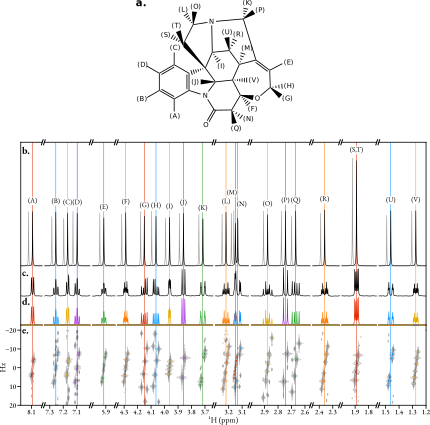
\includegraphics{strychnine_cupid/strychnine_cupid.pdf}
    \caption[
        Application of \acs{CUPID} on a simulated strychnine \acs{2DJ} dataset.
    ]
    {
        Application of \ac{CUPID} on a simulated strychnine \ac{2DJ} dataset.
        \textbf{a.} Black: the spectrum generated from \ac{FT} of the \ang{-45}
        signal. Grey: the spectrum of a simulated dataset with the same
        chemical shifts, with all scalar couplings set to \qty{0}{\hertz}.
        \textbf{b.} Conventional \ac{1D} spectrum.
        \textbf{c.} Multiplet structures assigned ($\epsilon =
        \nicefrac{\fswone}{\None} \approx \qty{0.39}{\hertz}$).
        \textbf{d.} Magnitude-mode \ac{2DJ} spectrum,
        with the locations of assigned oscillators given as coloured points.
    }
    \label{fig:strychnine-cupid}
\end{figure}
As a second example of applying \ac{CUPID} on simulated data, the chemical
shifts and isotropic scalar couplings associated with strychnine
were used to construct a 2DJ dataset. \ac{AWGN} was included with a target
\ac{SNR} of \qty{20}{\deci\bel}. The CUPID procedure was applied to filtered
sub-FIDs such that the signals arising from all spins were considered, with the
result presented in \cref{fig:strychnine-cupid}. There are numerous
regions in the dataset where strong coupling artefacts reside, and as such this
dataset provides a good gauge on the effectiveness of \ac{CUPID} when these are
present.

The \ac{MDL} was applied to the first direct-dimension \ac{FID} in order to
predict model order. In most circumstances, the model order used resulted
in estimation results in which the first-order signals were well
quantified, while those corresponding to strong coupling artefacts were neglected.
In some circumstances, certain strong couplings signals were quantified, though
the relevant oscillators were purged on every occasion based on the first-order
criteria. As such, no such artefacts appear in the final pure shift spectrum.
The absence of strong coupling artefacts in the estimation result also leads to
generated multiplet structures which do not exhibit the typical ``roofing''
phenomenon associated with strongly coupled spins (\textit{cf.} panels b and c of
\cref{fig:strychnine-cupid}). The clearest examples of this are
associated with the pair (U) \& (V), as well as trio (A), (B) \& (C). As with the
``four multiplets'' example, good agreement is achieved between the pure shift
spectrum generated via the \ang{-45} signal, and a spectrum generated by
running a \ac{1D} simulation with the same spin system, expect that scalar couplings
are set to \qty{0}{\hertz}.

\subsection{Quinine}
\begin{figure}
    \centering
    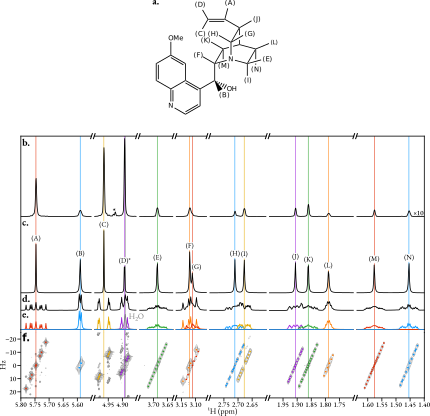
\includegraphics{quinine_cupid/quinine_cupid.pdf}
    \caption[
        Application of \acs{CUPID} on the non-aromatic regions of a quinine
        \acs{2DJ} dataset.
    ]{
        Application of \ac{CUPID} on the non-aromatic regions of a quinine
        \ac{2DJ} dataset.
        \textbf{a.} Spectrum produced using the \ang{45} shear and summation
        methodology. The peaks denoted by and asterisk arise from strong
        coupling artefacts.
        \textbf{b.} The spectrum generated from \ac{FT} of the \ang{-45}
        signal, with the signal arising from H\textsubscript{2}O (grey, close
        to \qty{4.9}{\partspermillion} neglected).
        \textbf{c.} Spectrum of the first direct-dimension signal in the
        \ac{2DJ} \ac{FID}.
        \textbf{d.} Multiplet structures assigned ($\epsilon =
        \nicefrac{\fswtwo}{\Ntwo} \approx \qty{0.92}{\hertz}$).
        \textbf{e.} Contour plot of the absolute value mode \ac{2DJ} spectrum,
        with the locations of assigned oscillators given as coloured points.
    }
    \label{fig:quinine-cupid}
\end{figure}

\Cref{fig:quinine-cupid} illustrates the result of applying \ac{CUPID} on
a dataset generated from a sample comprising quinine (\cref{fig:structures}.a)
in CD\textsubscript{3}OD,
with all signals arising from non-aromatic protons considered. The method
successfully generated a pure shift spectrum with distinct peaks for each
\textsuperscript{1}H environment.
An example of strong coupling artefacts being neglected can be seen
around the \qty{4.9}{\partspermillion} region, featuring signals from spins (C)
\& (D). As well as this, the multiplet grouping procedure is able to separate
the signals corresponding to spin (D) (purple) and residual water in the sample
(grey).
The presence of water is a hindrance since it heavily overlaps with (D)'s
multiplet structure.
To obtain a clean singlet for spin (D) in the pure shift spectrum, the
oscillator corresponding to the water signal was simply neglected from
the parameter set used to generate the \ang{-45} signal. This concept of
neglecting nuisance signals through post-processing has similarities with
\ac{SVD}-based approaches for solvent suppression\cite{Zhu1997}.
Solvent suppression approaches of this manner tend to operate by assuming
that the most significant component(s) in the data are derived from the
solvent, and these are subtracted from the dataset to
remove their influence. The removal of the water signal is slightly
different here, in that it was removed manually by inspecting the
\ac{CUPID} result. A knowledgeable user would be able to locate the water
signal, determine that it is unrelated to, and neglect it. In scenarios where
little is known about the sample, or the user does not have a high level or
expertise, manually neglecting signals in this manner may not be achievable.

This example provides a few examples where a noticeable under-fitting of
multiplet structures has occurred.
The most notable case comes from the spin (G) multiplet, where close proximity
with spin (F)'s multiplet has likely compounded the task of accurately
estimating the associated signals. With fewer oscillators than the true number
of signals at its disposal, the \ac{NLP} routine will compensate
by giving said oscillators large amplitudes and damping factors, so that they
can reasonably fit multiple similar-frequency signals. This phenomenon
culminates in the pure shift peak possessing an augmented linewidth.
This behaviour is also exhibited to a lesser extent by the multiplet for spin
(B), which comprises two pairs of very close signals in a dd structure. A
single oscillator is fit to each pair of signals, culminating in a broadened
pure shift peak.

For comparison, panel a of \cref{fig:quinine-cupid} presents a pure-shift
spectrum produced via application of a \ang{45} shear, followed by summation
along the indirect dimension. Due to the application of sine-bell apodisation,
the relative amplitudes of the pure-shift peaks are drastically different.
In particular, the alkenyl signals from spins (A), (C) \& (D), are less
perturbed by the apodisation relative to the aliphatic signals due to longer
$T_2$ times\footnote{
    Spins with longer $T_2$s produce signals which decay less rapidly.
    Sine-bell apodisation diminishes the amplitudes of the initial points in
    the \ac{FID}. Therefore, if the signal decays less rapidly, the relative
    extent by which the \emph{power} of the signal is diminished is less
    compared with a signal derived from a spin with a small $T_2$.
}. As well as this, signals arising from strong coupling between (C) and
(D) are visible (these are denoted with an asterisk).

\subsection{Camphor}
\begin{figure}%
    \centering%
    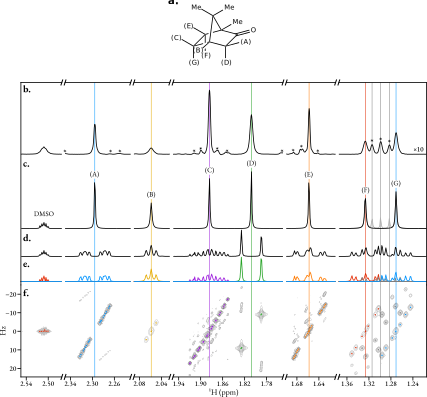
\includegraphics{camphor_cupid/camphor_cupid.pdf}%
    \caption[
        Application of \acs{CUPID} on a camphor dataset.
    ]{
        Application of \acs{CUPID} on camphor \ac{2DJ} dataset.
        \textbf{a.} Spectrum produced using the \ang{45} shear and summation
        methodology. The peaks denoted by and asterisk arise from strong
        coupling artefacts.
        \textbf{b.} Black: the spectrum generated from \ac{FT} of the \ang{-45}
        signal. Oscillators associated with strong coupling artefacts between
        spins (F) and (G) were neglected. Grey: spectrum generated without
        neglecting oscillators associated with strong coupling artefacts.
        \textbf{c.} Spectrum of the first direct-dimension \ac{FID}.
        \textbf{d.} Multiplet structures assigned ($\epsilon =
        \nicefrac{2 \fswtwo}{\Ntwo} \approx \qty{1.23}{\hertz}$).
        \textbf{e.} Magnitude-mode \acs{2DJ} spectrum, with the locations of
        assigned oscillators given as coloured points.
    }
    \label{fig:camphor-cupid}%
\end{figure}%
The application of \ac{CUPID} to the non-methyl signals of a \ac{2DJ}
dataset of camphor (\cref{fig:structures}.c) in \acs{DMSOd6} is presented
in \cref{fig:camphor-cupid}. As with the quinine example, a spectrum
generated through the shear and summation procedure is presented for
comparison. In most regions of the dataset, the estimation technique
successfully parametrised the first-order signals, while neglecting strong
coupling artefacts. However, it was not possible to solely estimate the
first-order signals associated with the pair of spins (F) and (G). The extent
of strong coupling between the nuclei is such that some of the strong coupling
artefacts have comparable amplitudes to the first-order signals. Reliance on
the
\ac{MMEMPM}\,---which determines the most significant components in
the data\,---therefore makes it challenging to solely estimate the first-order
signals in this case. The strong coupling signals which were estimated by the
routine are denoted in grey in the \SIrange{1.36}{1.24}{\partspermillion} region
of the spectrum. Their contributions to the spectrum of the \ang{-45} signal
are also plotted in grey. As with the shear and summation spectrum, three extra
peaks reside between the pure shift peaks associated with (F) and (G), which
ideally would not exist. In much the same way that the parameters associated
with water in the quinine example were neglected in constructing the \ang{-45}
signal, those associated with strong coupling artefacts can be too.
In neglecting said parameters, the black spectrum in panel b
results. Achieving this requires manual intervention, such that the user needs
the expertise to distinguish between first-order signals and strong coupling
artefacts.

\subsection{Dexamethasone}
\begin{sidewaysfigure}%
    \centering%
    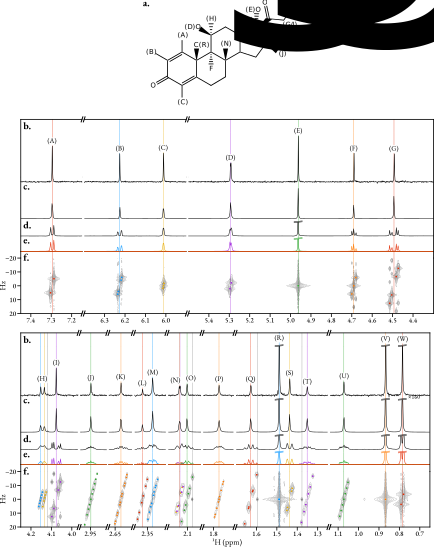
\includegraphics{dexamethasone_cupid/dexamethasone_cupid.pdf}%
    \caption[
        Application of \acs{CUPID} on a dexamethasone dataset.
    ]{
        Application of \acs{CUPID} on a \ac{2DJ} dataset of dexamethasone in
        \ac{DMSO}-d\textsubscript{6}.
        \textbf{a.} \acs{TSE-PSYCHE} spectrum of the sample.
        \textbf{b.} The spectrum generated from \ac{FT} of the \ang{-45}
        signal.
        \textbf{c.} Conventional \acs{1D} spectrum.
        \textbf{d.} Multiplet structures assigned ($\epsilon =
        \nicefrac{\fswtwo}{\Ntwo} \approx \qty{0.92}{\hertz}$).
        \textbf{e.} Magnitude-mode \acs{2DJ} spectrum, with the locations of
        assigned oscillators given as coloured points.
    }
    \label{fig:dexamethasone-cupid}%
\end{sidewaysfigure}%

\Cref{fig:dexamethasone-cupid} shows the result of applying CUPID on a
dataset acquired from a sample dexamethasone in DMSO-d\textsubscript{6}. A
pure shift spectrum was also acquired using the
\ac{TSE-PSYCHE} experiment\cite{Foroozandeh2018,Foroozandeh2015} for
comparison (see \cref{fig:tse_psyche}). Overall, excellent agreement is
achieved between the \ac{PSYCHE}
spectrum, and that generated using the \ang{-45} signal. The estimation routine
performed amicably in cases where heteronuclear coupling to
\textsuperscript{19}F were present. For spins (H) and (N), two distinct
multiplet structures were assigned, which are coloured blue and yellow (H) and
yellow and purple (N) in the figure. The perceptible though very small
heteronuclear coupling between \textsuperscript{19}F and (D) could not be
resolved by the estimation routine however.

In this example, there are a few cases where oscillators which result from
parametrising strong coupling artefacts exist. These persist because
either they have an indirect frequency $\approx \qty{0}{\hertz}$, or because at
least two parameterised artefacts are grouped together as part of the multiplet
assignment. As with the camphor example, a knowledgeable user could identify
and neglect the culprit oscillators if desired, though they are not purged in
producing the \ang{-45} signal in this case.

\note{Ask Ali: is PSYCHE quantitative? Quite major discrepancies in peak integrals}

\subsection{Estradiol}
\begin{figure}
    \includegraphics{estradiol_cupid/estradiol_cupid.pdf}%
    \caption[
        Application of \acs{CUPID} on a 17\textbeta-estradiol dataset.
    ]{
        Application of \acs{CUPID} on \ac{2DJ} dataset of 17\textbeta-estradiol
        in \acs{DMSOd6}.
        \textbf{a.} \acs{PSYCHE} spectrum of the sample (see
        \cref{fig:psyche} for details on the pulse sequence). The spectrum has
        been scaled such that its maximum is of the same magnitude as the
        spectrum in panel b.
        \ac{2DJ} dataset.
        \textbf{b.} Pure shift spectrum generated using \ac{CUPID}.
        \textbf{c.} Spectrum of the first direct-dimension \ac{FID} in the
        \textbf{d.} Multiplet structures assigned ($\epsilon =
        \qty{2}{\hertz}$).
        \textbf{e.} Magnitude-mode \ac{2DJ} spectrum, with coloured points
        denoting the frequencies of oscillators assigned using estimation.
        N.B. The \ac{2DJ} spectrum was produced using a more concentrated
        sample of estradiol, since the original \ac{2DJ} dataset was too
        insensitive to produce a useable spectrum after sine-bell apodisation.
    }
    \label{fig:estradiol-cupid}%
\end{figure}

A final showcase of \ac{CUPID} is provided by \cref{fig:estradiol-cupid},
where a low concentration (\qty{2}{\milli\molar}) sample of
17\textbeta-estradiol (\cref{fig:structures}.d) in \acs{DMSOd6} is
considered. This presents the most challenging example of using \ac{CUPID} due
to (a) the low \ac{SNR} and (b) the presence of incredibly complex regions for
a small molecule spectrum, featuring many overlapping multiplet structures.
Because of the complexity of the dataset, estradiol was used as a showcase of
the \ac{PSYCHE} experiment in the original work describing
it\cite{Foroozandeh2014}. With the sample and concentration and experimental
setup used, the \ac{PSYCHE} experiment produced a spectrum with very poor
\ac{SNR}, such that it is barely sensitive enough for pure shift peaks to be
distinguish from noise (panel a). However due to the innately higher
sensitivity associated with the \ac{2DJ} experiment (assuming similar
experiment parameters) it was still possible to generate a decent parameter
estimate of the \ac{2DJ} dataset. Due to the severe signal overlap in the first
direct-dimension \ac{FID}, initial values for the model order had to be
manually specified.  The time elapsed to run the estimation routine was rather
long, at \qty{10.25}{\minute} for all regions considered (see
\cref{tab:cupid-metrics} for a more detailed description of timings). This is
largely attributable to the high model orders, particularly in the most
downfield region (this region alone took over \qty{5.5}{\minute} to estimate).

\section{Summary}
In this chapter, \ac{CUPID}, a procedure for the construction of pure shift
spectra via the holistic estimation of \ac{2DJ} datasets, is presented.
Such spectra possess myriad beneficial features relative to alternative
methods, albeit with the requirement of a complex post-processing procedure.

% The original method for pure shift spectrum generation consisted of shearing a
% magnitude-mode \ac{2DJ} spectrum by \ang{45}, and computing the projection onto
% the $\Ftwo$ axis. To overcome the grotesque lineshapes which arise due to the
% presence of dispersion character, and non-linearities in the magnitude-mode
% spectrum, severe data treatment such as the used of sine-bell apodisation are
% applied. The resulting pure shift spectra suffer from reduced intensities
% because of this. On top of this, the intensities of peaks are attenuated by
% different extents, such that relative peak integrals become meaningless. The
% presence of strong coupling in the spin system also introduces unwanted
% artefacts into the spectra.

% Experimental procedures  based on ``chunking'' the initial sections of the
% \acp{FID} in a \ac{2D} experiment\,---\,including \ac{ZS}, \ac{BIRD} and
% \ac{PSYCHE}\,---\,have largely superseded the shear and summation approach.
% One key disadvantage of all of these is that only a fraction of the available
% spin magnetisation contributes to the final pure shift spectrum, leading to
% poorer sensitivity.

Through a number of examples, it has been shown that by employing parametric
estimation, a simple \ac{2DJ} experiment can be harnessed to generate pure
shift spectra with sharp absorption Lorentzian peaks which retain the same
signal intensity as the \ac{2DJ} experiment. \ac{CUPID} is able to perform
admirably even when state of the art techniques like \ac{PSYCHE} produce
spectra with such low \acp{SNR} as to render them unusable. Frequently, \ac{CUPID}
is able to automatically discard oscillators present in the model which either
correspond to strong coupling artefacts or noise, leading to simplified spectra
which appear to adhere to the weak coupling regime. There are cases where
strong coupling artefacts do end up in the estimation result. It has been shown
that there are circumstances where these can be manually neglected from the
parameter set to prevent them from having an unwanted influence on final pure
shift spectrum, though this requires manual intervention from a knowledgeable
user.

Simultaneously, \ac{CUPID} can assign multiplet structures,
by grouping oscillators which lie along a specific \ang{45} cross section in
frequency space. Achieving this experimentally\,---\,effectively involving
a \ac{2DJ} experiment in conjunction with a pure shift element\,---\,requires
running an extremely long (hours or even days) \ac{3D} pulse sequence. The
usefulness of the multiplet structures generated by \ac{CUPID} is dependent on
the level of the estimation routine's accuracy. On
numerous occasions within the examples presented here, the estimation routine
was unable to resolve certain, similar frequency signals. A complete
understanding of the coupling network associated with a given spin is not
attainable when this is so. However, such multiplet structures can still provide
valuable insights into the sample being studied.

\ac{CUPID} is limited by the complexity of the dataset of interest. The reasons
for this are two-fold. First, for datasets comprising progressively more peaks
in a given spectral region, the difficulty in generating accurate parameter
estimates becomes harder. Second, with an increased model order required to
estimate the dataset, the computation time increases drastically.
This feature is most clearly observed when comparing the times required in
estimating the different regions considered in the estradiol example. As a rule
of thumb, it is anticipated that \ac{CUPID} will perform admirably on datasets
derived from small molecules, though datasets derived from large molecules such
as proteins are likely to be too complex and demanding for good results.

